\fancyhead[LE,RO]{Investigating a ternary system -- ,,TER''}
\fancyhead[LO,RE]{\thesection}
\fancyfoot[LE,RO]{\thepage}
\fancyfoot[RE,LO]{\emph{Physical chemistry laboratory practice}}

\section{Investigating a ternary system}
\subsection{Introduction}

Ternary systems pose interesting questions not only form a theoretical point of view, but they also have practical importance for instance in metallurgy or the plastic industry. Just consider alloys, in which several different solid phases could be present, or mutually insoluble liquid phases which contain a common dissolved substance, for instance a drug dissolved in fat and water. In a ternary system, the mutual solubility of the components could be different. In every ternary system there is a pressure and/or temperature at which at least two components are only partially soluble in each other. The presence of a third component -- in case it mixes partially or completely in the other two -- could modifiy the mutual solubility of the two other components.

If the components are not reacting with each other, then to describe the state of a ternary system, knowing the temperature and the pressure is necessary. Since knowing the molefraction of two components determines the molefraction of third, the degree of freedom in such a system is 4. Therefore, at a given temperature and pressure, we only have to know the molefraction of two of the components to know the exact state of the system. To plot the phase diagram of a ternary system on a plane, it is useful to take pressure and temperature constant. By doing this, the phase diagram of the system can be plotted on an equilateral triangle. The corners of the triangle represent a system composed of only one of the three components. For easier reading, there is a convention regarding the orientation of the axes of the ternary triangle; it is always counter-clockwise. The sides (axes) of the triangle, the mole or weigth fraction or percentage of the components are represented (Fig. \ref{fig:1}.).

\begin{figure}[b!]
\centering
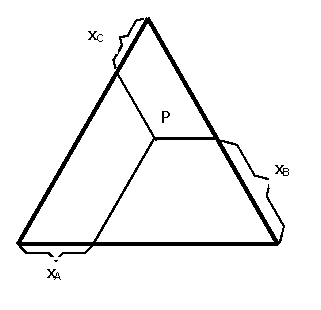
\includegraphics{fig/terner1.eps}
\caption{Composition of a ternary system on a ternary diagram. The mole fraction of the components increases couter-clockwise.}
\label{fig:1}
\end{figure}

Point \emph{,,P''} inside the triangle represents a system with all three components. We can read the composition by finding the respective molefraction values on the axes. The sides give the composition of the pairwise two-component systems as well (Fig. \ref{fig:2} I.). In Fig. \ref{fig:2}. (I.) we show the composition of a ternary system, in which two components mix partially (water--chloroform), while the third (acetic acid for instance) dissolves completely in both. The area below the curve marks the heterogeneous systems. In such a state, the system will have two, so-called \emph{,,conjugated phases''}. Any point in the triangle outside of this area represents a homnogeneous system. Where the curve intersects any side of the triangle, the system has two components; x$_{A,1}$ and x$_{C,1}$ mean the solubility of water in chloroform, x$_{A,2}$ and x$_{C,2}$ mean the solubility of chloroform in water, if A is water, B is acetic acid and C is chloroform. If all the component pairs are only partially soluble in each other, then we get a diagram similar to Fig. \ref{fig:2}. (II.).

\begin{figure}
\centering
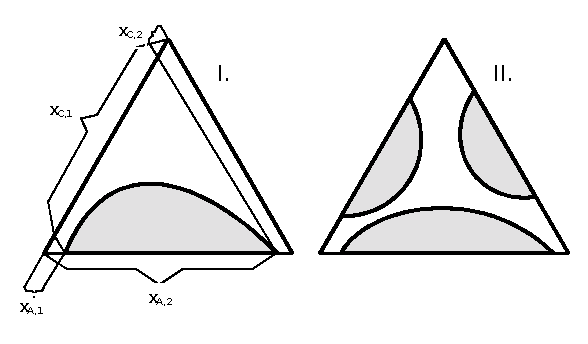
\includegraphics{fig/terner2.eps}
\caption{Phase diagrams of ternary systems. (I.) Only one component pair is partially miscible: the gray area under the curve is heterogeneous, the rest (white area) is homogeneous. (II.) All three component pairs are only partially miscible in each other.}
\label{fig:2}
\end{figure}


From now on we discuss the water--chloroform--acetic acid ternary system. As we have mentioned already, any point below the curve will mean a system with two conjugated phases. Connecting the two points that are representing the conjugated phases we get the so called \emph{,,tie line''}. All the tie lines will have a common intersection, usually outside of the triangle (point \emph{P}, Fig. \ref{fig:3}). The tie lines are usually not parallel with the base of the triangle, because the third component doesn't dissolve equally in the two conjugated phases. Drawing a tangent from pont P to the curve we get point \emph{K}, the \emph{plait point} for a given temperature and pressure. If not all one but two or three component pairs are only partially miscible in each other, the we get two or three plait points, respectively. In the practice we will investigate the water-chloroform-acetic acid ternary system. 

\begin{figure}
\centering
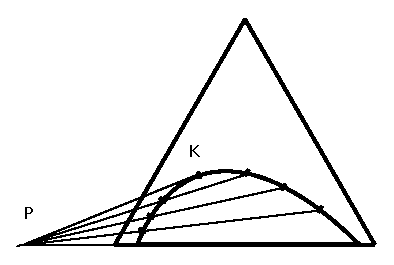
\includegraphics{fig/terner3.eps}
\caption{Determining the plait point in a system in which only one component pair's solubility is limited. P: intersection of the tie lines. K: plait point.}
\label{fig:3}
\end{figure}


\subsection{Practice procedures}

Prepare 20 cm$^3$ 15, 30, 50, 60, 70, 80, 85, 90 and 95 volume\% mixtures of chloroform and acetic acid. The volume\% is given with respect to chloroform. Measure the components with an automatic burette into clean, water-free Erlenmeyer flasks, and close them. Titrate the mixtures with water using a graduated (0.05 cm$^3$) 10 cm$^3$ automatic burette until you observe a slight opaque white color throughout the mixture. Find the density of the components from the table below, and using these and the volumes used until the endpoints (opaque color) calculate the mole fraction and mass fractoin of all three components for all 9 mixtures. Draw the two phase diagrams, using both mole and mass fraction as well (two separate diagrams) to get the equilibrium diagram. Give the results of the calculations in a table such as the following:

\begin{table}[h!]
\centering
\begin{tabular}{|l|l|l|l|l|l|l|l|l|l|l|l|}
\hline
\multicolumn{4}{|c|}{\begin{tabular}[c]{@{}l@{}}organic solvent\\ M = ... g mole$^{-1}$\\ $\rho$ = ... g cm$^{-3}$ \end{tabular}} & \multicolumn{4}{|c|}{\begin{tabular}[c]{@{}l@{}}weak acid\\ M = ... g mole$^{-1}$\\ $\rho$ = ... g cm$^{-3}$ \end{tabular}}  & \multicolumn{4}{|c|}{\begin{tabular}[c]{@{}l@{}}water\\ M = ... g mole$^{-1}$\\ $\rho$ = ... g cm$^{-3}$ \end{tabular}}  \\ \hline
cm$^3$                        & mole                        & x                        & m\%                        & cm$^3$    & mole    & x   & m\%   & cm$^3$   & mole   & x  & m\%  \\ \hline
2                          &                             &                          &                            &        &         &     &       &       &        &    &      \\ \hline
4                          &                             &                          &                            &        &         &     &       &       &        &    &      \\ \hline
...                        &                             &                          &                            &        &         &     &       &       &        &    &      \\ \hline
\end{tabular}
\end{table}


To determine the plate point, prepare a mixture which has two conjugated phases (system under the curve). Separate them, and titrate a known mass of both of them with NaOH to get the mass of acetic acid in both of them. Then calculate the mass fraction of acetic acid in the conjugated phases. After this step we can draw a tie line. Repeat it with another mixture with different composition, to get an additional tie line. Draw a tangent from the intersection of the tie lines to get the plait point. Give the mass fraction composition of this point as a final result of the practice.

Recommendations for the two systems:

\begin{itemize}
\item A: 20 ml water, 25 ml chloroform, 1 ml acetic acid
\item B: 25 ml water, 25 ml chloroform, 3 ml acetic acid
\end{itemize}

Close the flasks, shake them for about 5 minutes to reach equilibrium. Separate the phases in a separation funnel, and titrate 5 ml of the organic and 10 ml of the water phase, after measuring the mass of both. Use either 0.1 M or 1 M NaOH fot titration and a few drops of phenolphthalein as indicator. Prepare the following table:

\begin{table}[h!]
\centering
\begin{tabular}{|l|l|l|l|l|l|}
\hline
phase & \begin{tabular}[c]{@{}l@{}}titrant volume (ml)\\ for organic phase\end{tabular} & m$_{acid}$ (g) & m$_{phase}$ (g) & m\% \\ \hline
A organic      & & & &  \\ \hline
A water        & & & &  \\ \hline
B organic      & & & &  \\ \hline
B water        & & & &  \\ \hline
\end{tabular}
\end{table}


Knowing the mass of the phases you can calculate the mass fraction of acetic acid in both phases. Using these, find the intersection with the equlibrium line to get the conjugated phases' composition. Draw both tie lines. Find point P, the intersection of the tie lines. Draw the tangent to the equilibrium line from point P, to get the plait point K. Read the mass fraction composition of the plait point and write it down in your notebook as a final conclusion.  



\begin{table}[]
\centering
\caption{Solvent molar mass and density.}
\begin{tabular}{rcc}
\multicolumn{1}{l}{}                                & \multicolumn{1}{c}{\begin{tabular}[c]{@{}c@{}}M\\ g mole$^{-1}$\end{tabular}} & \multicolumn{1}{c}{\begin{tabular}[c]{@{}c@{}}Density at 20 $^o$C\\ g cm$^{-3}$\end{tabular}} \\ \hline
\begin{tabular}[c]{@{}r@{}}acetic acid\end{tabular} & 60.05                                                                     & 1.0497                                                                                 \\ \hline
chloroform                                            & 119.38                                                                    & 1.4891                                                                                 \\ \hline
water                                                 & 18.02                                                                     & 0.9982                                                                                
\end{tabular}
\end{table}

%\begin{figure}
%\includegraphics{fig/ternary_diagram.pdf}
%\end{figure}
%\begin{tikzpicture}
%\begin{ternaryaxis}[
%	%title=The water--chloroform--acetic acid ternary system,
%	xlabel=Weight percent of acetic acid,
%	ylabel=Weight percent of chloroform,
%	zlabel=Weight percent of water,
%	label style=sloped,
%	area style,
%]
%	\addplot3 table {
%	0 0.1 0.9
%	 
%	0.28 0.35 0.37
%	0.25 0.6 0.15
%	0.1 0.9 0
%	0 1 0
%	0 0 1
%	};
%	%\addlegendentry{$\gamma$FeNi}
%
%	%\node[inner sep=0.5pt,circle,draw,fill=white,pin=-15:\footnotesize Stainless Steel] at (axis cs:0.18,0.74,0.08) {};
%	
%\end{ternaryaxis}
%\end{tikzpicture}



